%%Intro to the Literature Review
    The study of ladder lottieres as mathematical objects began in 2010, in  the paper
    \textbf{Efficient Enumeration of Ladder Lotteries and its Application}. The paper was 
    written by four authors, Yamanaka, Horiyama, Uno and Wasa. In this paper the 
    authors present an algorithm for generating all the ladder lotteries of an 
    arbitrary permutation, $\pi$. Since this paper emerged, there have been 
    several other paper written directly about ladder lotteries. 
    These papers include \textbf{The Ladder Lottery Realization Problem},
    \textbf{Optimal Reconfiguration of Optimal Ladder Lotteries}, 
    \textbf{Efficient Enumeration of all Ladder Lotteries with K Bars},
    \textbf{Coding Ladder Lotteries} and
    \textbf{Enumeration, Counting, and Random Generation of Ladder Lotteries}.

%$input review of first paper
\section{Efficient Enumeration of Ladder Lotteries and its Application}

%%Intro
In the Efficient Enumeration of Ladder Lotteries and its Application, written by Matsui, Nakada, Nakano Uehara and Yamanaka,
the authors provide an algorithm for generating $OptL\{\pi\}$ 
for any $\pi$, in $\mathcal{O}(1)$ per ladder~\cite{A1}. The authors refer to this algorithm as {\sc FindAllChildren}
which can be found in Algorithm~\ref{Alg:FindAllChildren}. 
\begin{algorithm}[!htp]
	\begin{algorithmic}[1]
		\Function{FindAllChildren}{$ladder$, $cleanLevel$, $n$}
			\State $currentRoute \gets n$
			\While{$currentRoute \geq cleanLevel$}
				\State going top left to bottom right 
				\For{$bar \in currentRoute$}
					\State $row \gets$ row of $bar$ in $ladder$ 
					\State $col \gets$ col of $bar$ in $ladder$
					\State $lowerNeighbor \gets ladder[row-1][col]$
					\If{$lowerNeighbor$ is right swappable}
						\State {\sc RightSwap($ladder$, $bar$, $lowerNeighbor$)}
						\State {\sc {\sc FindAllChildren}($ladder$, $y+1$, $n$)}
						\State {\sc LeftSwap($ladder$, $bar$, $lowerNeighbor$)}
					\EndIf
				\EndFor
				\State $currentRoute \gets currentRoute-1$
			\EndWhile
			\State $currentRoute \gets cleanLevel-1$
			\For{$bar \in currentRoute$}
				\State $row \gets$ row of $bar$ in $ladder$ 
				\State $col \gets$ col of $bar$ in $ladder$
				\State $lowerNeighbor \gets ladder[row-1][col]$
				\If{$lowerNeighbor$ is right swappable \textbf{and} is the rightmost bar of $currentRoute-1$}
					\State {\sc RightSwap($ladder$, $bar$)}
					\State {\sc FindAllChildren($ladder$, $cleanLevel$, $n$)}
					\State {\sc LeftSwap($ladder$, $bar$)}
				\EndIf
			\EndFor
		\EndFunction
	\end{algorithmic}
	\caption{The algorithm for listing $OptL\{\pi\}$.}
	\label{Alg:FindAllChildren}
\end{algorithm}
\pagebreak

One will note that two helper functions, {\sc RightSwap} and {\sc LeftSwap}, are required to complete 
{\sc FindAllChildren}. The details of these algorithms are not found 
in the paper~\cite{A1}. Thus, these algorithms and their details can be found in the Appendix in Algorithm \ref{Alg:RightSwap}
and Algorithm \ref{Alg:LeftSwap}.
{\sc FindAllChildren} is the first algorithm for generating $OptL\{\pi\}$.\newline
{\sc FindAllChildren} enumerates $OptL\{\pi\}$ as a tree of ladders.

%%Put this in the Appendix

%%DONE PUT IN Appendix

%%%%%%%%%%%%%%%%%%%%%%%%%%%%%%%FIND ALL CHILDREN ALGORITHM%%%%%%%%%%%%%%%%%%%%%%%%%%%%%



%%%%%%%%%%%%%%%%%%END ALGORITHM%%%%%%%%%%%%%%%%%%%%%%%%%%



{\sc FindAllChildren} was used in this thesis to generate the sample data that aided in finding solutions for 
the Gray Code Problem in Chapter 3 and the Minimum Height Problem in Chapter 4.  
Therefore, this algorithm is paramount for the findings of this thesis. 
To see the tree structure generated by {\sc FindAllChildren} for $OptL\{(4,3,2,1)\}$ 
please refer to Figure~\ref{Fig:TreeFAC}. 
\begin{figure}[h]
	\centering 
	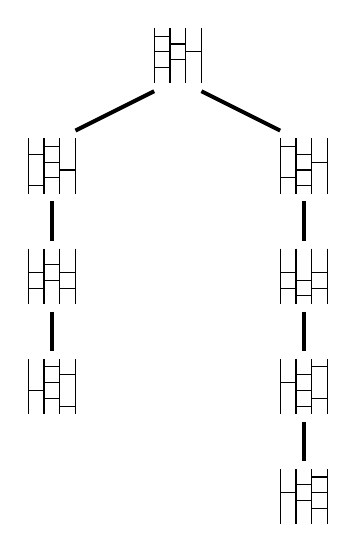
\begin{tikzpicture}
		%%L1
		\draw(5, 10) to (5, 9.3);
			\draw(5, 9.9) to (5.2, 9.9);
			\draw(5.2, 9.8) to (5.4, 9.8);
			\draw(5.4, 9.7) to (5.6, 9.7);
		\draw(5.2, 10) to (5.2, 9.3);
			\draw(5, 9.7) to (5.2, 9.7);
			\draw(5.2, 9.6) to (5.4, 9.6);
		\draw(5.4, 10) to (5.4, 9.3);
			\draw(5, 9.5) to (5.2, 9.5);
		\draw(5.6, 10) to (5.6, 9.3);
		%L2
		\draw[line width = .5mm](5, 9.2) to (4, 8.7);
		\draw[line width = .5mm](5.6, 9.2) to (6.6, 8.7);
			%%L2
			\draw(3.4, 8.6) to (3.4, 7.9);
				\draw(3.4, 8.4) to (3.6, 8.4);
				\draw(3.4, 8) to (3.6, 8);
			\draw(3.6, 8.6) to (3.6, 7.9);
				\draw(3.6, 8.5) to (3.8, 8.5);
				\draw(3.6, 8.3) to (3.8, 8.3);
				\draw(3.6, 8.1) to (3.8, 8.1);
			\draw(3.8, 8.6) to (3.8, 7.9);
				\draw(3.8, 8.2) to (4, 8.2);
			\draw(4.0, 8.6) to (4.0, 7.9);

				%%level
				\draw[line width = .5mm](3.7, 7.8) to (3.7, 7.3);
			\draw(3.4, 7.2) to (3.4, 6.5);
				\draw(3.4, 6.9) to (3.6, 6.9);
				\draw(3.4, 6.7) to (3.6, 6.7);
			\draw(3.6, 7.2) to (3.6, 6.5);
				\draw(3.6, 7) to (3.8, 7);
				\draw(3.6, 6.8) to (3.8, 6.8);
			\draw(3.8, 7.2) to (3.8, 6.5);
				\draw(3.8, 6.9) to (4, 6.9);
				\draw(3.8, 6.7) to (4, 6.7);
			\draw(4.0, 7.2) to (4.0, 6.5);

		%%L3
			\draw(6.6, 8.6) to (6.6, 7.9);
				\draw(6.6, 8.5) to (6.8, 8.5);
				\draw(6.8, 8.4) to (7, 8.4);
				\draw(7, 8.3) to (7.2, 8.3);
			\draw(6.8, 8.6) to (6.8, 7.9);
				\draw(6.8, 8.2) to (7, 8.2);
				\draw(6.8, 8) to (7, 8);
			\draw(7, 8.6) to (7, 7.9);
				\draw(6.6, 8.1) to (6.8, 8.1);
			\draw(7.2, 8.6) to (7.2, 7.9);
			
			
			\draw[line width = .5mm](6.9, 7.8) to (6.9, 7.3);

			\draw(6.6, 7.2) to (6.6, 6.5);
				\draw(6.6, 6.9) to (6.8, 6.9);
				\draw(6.6, 6.7) to (6.8, 6.7);
			\draw(6.8, 7.2) to (6.8, 6.5);
				\draw(6.8, 6.8) to (7, 6.8);
				\draw(6.8, 6.6) to (7, 6.6);
			\draw(7.0, 7.2) to (7.0, 6.5);
				\draw(7, 6.9) to (7.2, 6.9);
				\draw(7, 6.7) to (7.2, 6.7);
			\draw(7.2, 7.2) to (7.2, 6.5);

			\draw[line width = .5mm](3.7, 6.4) to (3.7, 5.9);

			\draw(3.4, 5.8) to (3.4, 5.1);
				\draw(3.4, 5.4) to (3.6, 5.4);
			\draw(3.6, 5.8) to (3.6, 5.1);
				\draw(3.6, 5.7) to (3.8, 5.7);

				\draw(3.6, 5.5) to (3.8, 5.5);
				\draw(3.6, 5.3) to (3.8, 5.3);
			\draw(3.8, 5.8) to (3.8, 5.1);
				\draw(3.8, 5.6) to (4, 5.6);
				\draw(3.8, 5.2) to (4, 5.2);
			\draw(4.0, 5.8) to (4.0, 5.1);

			\draw[line width = .5mm](6.9, 6.4) to (6.9, 5.9);

			
			\draw(6.6, 5.8) to (6.6, 5.1);
				\draw(6.6, 5.5) to (6.8, 5.5);
			\draw(6.8, 5.8) to (6.8, 5.1);
				\draw(6.8, 5.6) to (7, 5.6);

				\draw(6.8, 5.4) to (7, 5.4);
				\draw(6.8, 5.2) to (7, 5.2);
			\draw(7.0, 5.8) to (7.0, 5.1);
				\draw(7.0, 5.7) to (7.2, 5.7);
				\draw(7.0, 5.3) to (7.2, 5.3);
			\draw(7.2, 5.8) to (7.2, 5.1);

			\draw[line width = .5mm](6.9, 5) to (6.9, 4.5);

			\draw(6.6, 4.4) to (6.6, 3.7);
				\draw(6.6, 4.1) to (6.8, 4.1);
			\draw(6.8, 4.4) to (6.8, 3.7);
				\draw(6.8, 4.2) to (7, 4.2);

				\draw(6.8, 4) to (7, 4);
			\draw(7.0, 4.4) to (7.0, 3.7);
				\draw(7.0, 4.3) to (7.2, 4.3);
				\draw(7.0, 4.1) to (7.2, 4.1);
				\draw(7.0, 3.9) to (7.2, 3.9);
			\draw(7.2, 4.4) to (7.2, 3.7);



	\end{tikzpicture}
	\caption{The tree structure of $OptL\{(4,3,2,1)\}$ generated by {\sc FindAllChildren}}
	\label{Fig:TreeFAC}
\end{figure}
\pagebreak
{\sc FindAllChildren} is based on several key concepts. One of which is the local swap operation 
which has already been discussed. The next fundamental concept is the \emph{route} of an element, 
which is the sequence of bars the element travels along in order to reach its final position in the 
sorted permutation. The bars are read from top to bottom. For every bar, two elements cross 
the bar, therefore the bar is associated with the route of the greater of the two elements~\cite{A1}. 
In Figure~\ref{Fig:Route} the route of element $4$ is the sequence of bars 
$(4,1),(4,2),(5,4)$. To see the route of an element please refer to Figure~\ref{Fig:Route}. When a 
right swap operation occurs, the bar of the route associated with a lesser element is 
swapped above two bars of a route associated with a greater element. For example, in Figure~\ref{fig:rightSwap} in the right ladder, 
the bar $(3,1)$ which is associated with the route of element $3$ is right swapped above the two bars $(5,1)$ and $(5,3)$ 
both of which are associated with the route of $5$.\par 
\begin{figure}[h]
	\centering
	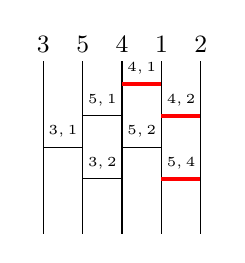
\begin{tikzpicture}
		\draw(0, 0) to (0, 2.2);
			\node at(.25, 1.3){\tiny{$3,1$}};
			\draw(0, 1.1) to (.5, 1.1);
		\draw(.5, 0) to (.5, 2.2);
			\node at(.75, 1.7){\tiny{$5,1$}};
			\draw(.5, 1.5) to (1, 1.5);
			\node at(.75, .9){\tiny{$3,2$}};
			\draw(.5, .7) to (1, .7);
		\draw(1, 0) to (1, 2.2);
			\node at(1.25, 2.1){\tiny{$4,1$}};
			\draw[line width=.5mm, red ](1, 1.9) to (1.5, 1.9);
			\node at(1.25, 1.3){\tiny{$5,2$}};
			\draw(1, 1.1) to(1.5, 1.1);
		\draw(1.5, 0) to (1.5, 2.2);
			\node at(1.75, 1.7){\tiny{$4,2$}};
			\draw[line width=.5mm, red ](1.5, 1.5) to (2, 1.5);
			\node at(1.75, .9){\tiny{$5,4$}};
			\draw[line width=.5mm, red ](1.5, .7) to (2, .7);
		\draw(2, 0) to (2, 2.2);


		\node at(0.0, 2.4){\small{$3$}};
		\node at(0.5, 2.4){\small{$5$}};
		\node at(1.0, 2.4){\small{$4$}};
		\node at(1.5, 2.4){\small{$1$}};
		\node at(2.0, 2.4){\small{$2$}};
	\end{tikzpicture}
	\caption{The route of element 4=(4,1),(4,2),(5,4).}
	\label{Fig:Route}
\end{figure}



The \emph{clean level} is defined as one more than the largest 
element associated with any bar that has undergone a right swap operation. 
For example, if the largest element associated with a bar that has undergone a 
right swap operation is element $4$, then the clean level is $5=4+1$.
 Please refer to Figure~\ref{Fig:CleanLevel} for an example of the clean level.
 If no bars have been right swapped, then the clean level is $1$.
If the largest element to have undergone a right swap operation is the maximal element in $\pi$, 
then the clean level is $max+1$.\pagebreak

\begin{figure}[t]
	\centering 
	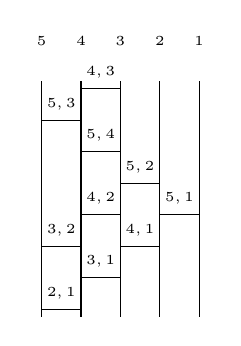
\begin{tikzpicture}
		\draw(0, 0) to (0, 3);
			\node at(.25, 2.7){\tiny{$5,3$}};
			\node at(.25, 1.1){\tiny{$3,2$}};
			\node at(.25, .3){\tiny{$2,1$}};
			\draw(0, 2.5) to (.5, 2.5);			
			\draw(0, .9) to (.5, .9);
			\draw(0, .1) to (.5, .1);

		\draw(.5, 0) to (.5, 3);
			\node at(.75, 3.1){\tiny{$4,3$}};
			\node at(.75, 2.3){\tiny{$5,4$}};
			\node at(.75, 1.5){\tiny{$4,2$}};
			\node at(.75, .7){\tiny{$3,1$}};

			\draw(.5, 2.9) to (1, 2.9);
			\draw(.5, 2.1) to (1, 2.1);
			\draw(.5, 1.3) to (1, 1.3);
			\draw(.5, .5) to (1, .5);
		\draw(1, 0) to (1, 3);
			\node at(1.25, 1.9){\tiny{$5,2$}};
			\node at(1.25, 1.1){\tiny{$4,1$}};

			\draw(1, 1.7) to (1.5, 1.7);
			\draw(1, .9) to (1.5, .9);
		\draw(1.5, 0) to (1.5, 3);
			\node at(1.75, 1.5){\tiny{$5,1$}};
			\draw(1.5, 1.3) to (2, 1.3);
		\draw(2, 0) to (2, 3);

		%%%%%%%%%%%%%%%%%%%%%%%%%%%%
		\node at(0, 3.5){\tiny{$5$}};
		\node at(.5, 3.5){\tiny{$4$}};
		\node at(1, 3.5){\tiny{$3$}};
		\node at(1.5, 3.5){\tiny{$2$}};
		\node at(2, 3.5){\tiny{$1$}};
\end{tikzpicture}
	\caption{A ladder with a clean level of $6$. The largest element whose associated bars have undergone a right swap operation is $5$}
	\label{Fig:CleanLevel}
\end{figure}


Each $OptL\{\pi\}$ has a unique ladder with a clean level of one. This ladder 
is known as the \emph{root ladder}. The root ladder is the root of the tree structure 
produced from {\sc FindAllChildren}. Unlike every other ladder in the tree, 
the root ladder cannot be derived from a local swap operation. Thus, the root ladder 
must be created by another algorithm other than {\sc FindAllChildren}. 
The authors do not provide details on how to create the root ladder. Thus, an 
algorithm for creating the root ladder can be found in the Appendix in Algorithm~\ref{Alg:RootLadder}.
The details of the root ladder are also explained in the Appendix.
Given all permutations of order $n$, the root ladder for the descending permutation requires 
the most rows. 
\begin{theorem}
  The number of rows required for the root ladder of the descending permutation is $2(n-1) - 1$.
\end{theorem}
\begin{proof}
  The number of rows for the ladder data-structure is calculated a follows: When a bar is added to the ladder it can be added 
  to an already existing row or to a new row. 
  If the current state of the ladder is empty then adding the first bar produces the second ladder in
  $L_{n}$. Since the bars are being added bottom right to top left, and the first bar to be added belongs 
  to the $nth$ route, then it must be added to $row=n-1$, $col=n-1$. As bars of the $nth$ route get 
  continuously added to the ladder, each bar is added a row above the previous bar and to a column 
  to the left of the column of the previous bar.
  Since no two bars of the $nth$ route can be on the same row, this will require $n-1$ rows. Note, if they were added to the same 
  row, then the left end point of the right bar would be touching the right end point of the left bar which is disallowed. Once the 
  bars of the $nth$ element are added, the bars of the $n-1th$ route will be added. The $n-1th's$ first bar 
  will be added to the $n-2$ column, otherwise it would be directly below the first bar of the $nth$ route, which is a violation. 
  Since the first bar of the $n-1$'s element is added to column $n-2$, then it must be given a new row, otherwise its right end point 
  will be touching  the left end point of the first bar of route $n$. The remaining $n-2$ bars of element $n-1$
  will be added bottom right to top left, but none of their end points will touch the end points of element $n$ seeing as they will 
  always be two columns apart from any bar in $n's$ route. The same logic applies to element $n-2$, it will require one extra row for its 
  first bar, in order not to touch the first bar of element $n-1$, but the remainder of its bars will always be two columns away from 
  the remainder of the bars for $n-1$, etc. Therefore there are $n-1$ rows required for the $nth$ element and each subsequent 
  element, $k$ requires only one new row. Since $2 \leq k < n$, then there are $(n-2)$ additional rows required for the ladder. Note that element 
  $1$ has no bars in its route. Therefore there are $(n-1)$ rows required for element $n's$ bars  plus $(n-2)$ rows required for 
  all the remaining $2 \leq k < n$ routes. In conclusion the number of rows required is $(n-1) + (n-2) = 2(n-1)-1$. 
  See figure for the tree of ladders 
  generated by {\sc ModifiedSJT} for $n=4$. Note that the maximum number of rows required is $2(n-1)-1=2(3)-1=5$.
\end{proof}



%%Root ladder subsection




%%DONE Appendix SECTION

In concluding the section on the enumeration problem, we have analyzed the original paper along with 
making additions to the algorithm {\sc FindAllChildren} by providing four essential algorithms 
for the completion of {\sc FindAllChildren}. The algorithms are Algorithm~\ref{Alg:RootLadder}, Algorithm~\ref{Alg:RightSwap},
Algorithm~\ref{Alg:LeftSwap} and Algorithm~\ref{Alg:ShiftSubLadder} which can be found in the Appendix. In concert, these five algorithms solve the enumeration 
problem which lists $OptL\{\pi\}$ in $O(1)$ time per ladder. 


\pagebreak

%%input revoiew of second paper


\subsection{Ladder-Lottery Realization}

In their paper \textbf{Ladder-Lottery Realization} the authors provide 
a rather interesting puzzle in regards to ladder lotteries. The puzzle 
is known as the ladder-lottery realization problem. In order to understand
the problem, one must know what a \emph{multi-set} is. A \emph{multi-set}
is a set in which an element appears more than once. The exponent 
above the element indicates the number of times it appears in the set.
For example, given the following multi-set, $\{3^{2}, 2^{4}, 5^{1}\}$ 
the element $3$ appears twice in the set, the element $2$ appears four times
in the set and the element $5$ appears once in the set.
The ladder-lottery realization puzzle asks, given an arbitrary starting permutation 
and a multi-set of bars, 
is there a \emph{non-optimal} ladder lottery for the arbitrary permutation
that uses every bar in the multi-set the number 
of times it appears in the  multi-set. 
For an example of an affirmative solution to the ladder lottery realization problem, see Fig. 2.4.


\begin{figure}[!htp]
    \begin{center}
        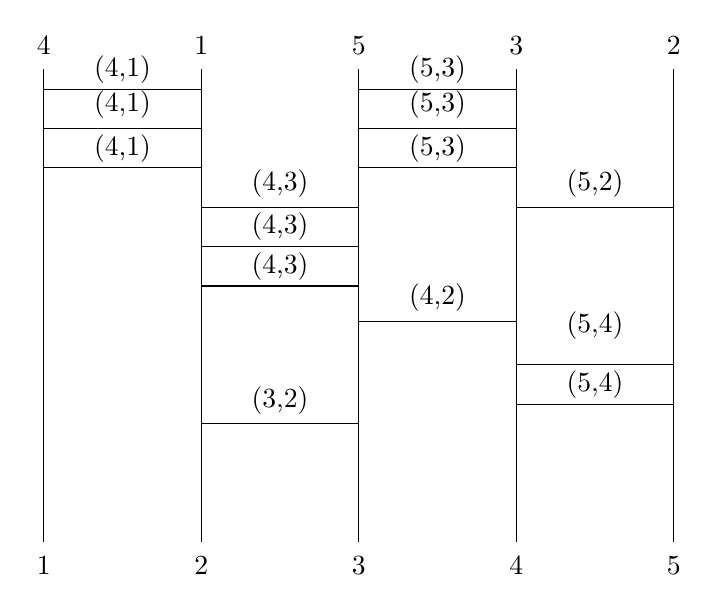
\begin{tikzpicture}
            \draw (0, 0) to (0, 6);
                \node at(0, -0.3){1};
                \node at(0, 6.3){4};
            \draw(2, 0) to (2, 6);
                \node at(2, -0.3){2};
                \node at(2, 6.3){1};
            \draw(4, 0) to (4, 6);
                \node at(4, 6.3){5};
                \node at(4, -0.3){3};
            \draw(6, 0) to (6, 6);
                \node at(6, 6.3){3};
                \node at(6, -0.3){4};
            \draw(8, 0) to (8, 6);
                \node at(8, 6.3){2};
                \node at(8, -0.3){5};

            %%draw the bars
                \node at(1, 6){(4,1)};
                    \draw(0, 5.75) to (2, 5.75);
            \draw(0, 5.25) to (2, 5.25);
                \node at(1, 5.55){(4,1)};
            \draw(0, 4.75) to (2, 4.75);
                \node at(1, 5){(4,1)};

            \draw(4, 5.75) to (6, 5.75);
                \node at(5, 6){(5,3)};
            \draw(4, 5.25) to (6, 5.25);
                \node at(5, 5.55){(5,3)};
            \draw(4, 4.75) to (6, 4.75);
                \node at(5, 5){(5,3)};

            \draw(2, 4.25) to (4, 4.25);
                \node at (3, 4.55){(4,3)};
            \draw(2, 3.75) to (4, 3.75);
                \node at (3, 4){(4,3)};
            \draw(2, 3.25) to (4, 3.25);
                \node at (3, 3.5){(4,3)};
            
            \draw(2, 1.5) to (4, 1.5);
                \node at(3, 1.8){(3,2)};
            
            \draw(4, 2.8) to (6, 2.8);
                \node at (5, 3.1){(4,2)};
            \draw(6, 4.25) to (8, 4.25);
                \node at (7, 4.55){(5,2)};
            
            \draw(6, 2.25) to (8, 2.25);
                \node at (7,2.75){(5,4)};
            
            \draw(6, 1.75) to (8, 1.75);
                \node at (7, 2){(5,4)};
            
        \end{tikzpicture}
    \end{center}
      


    \caption{An affirmative solution to the Ladder Lottery Realization Problem given a starting perumtation $(4,1,5,3,2)$ and the multi set of bars $\{(4,1)^{3}, (4,3)^{3}, (4,2)^{1}, (5,4)^{2}, (5,3)^{3}, (5,2)^{1},(3,2)^{1}\}$}
\end{figure}
\pagebreak
The authors prove that the ladder-lottery realization problem in NP-Hard
by reducing the ladder-lottery realization to the One-In-Three 3SAT, 
which has already been proven to be NP-Hard. The One-In-Three 3SAT 
problem is a problem such that given a set of variables $(X)$, a collection 
of \emph{disjuntcive clauses} $(C)$ which are disjunctive expressions over 
literals of $X$. Each clause in $C$ 
must contain three literals then is there a truth assignment for $X$ such that 
each clause in $C$ has exactly one true literal. For eaxmple, let 
$X=\{p, q, r, s, t\}$ and let $C=\{C_{p,q,s}, C_{r,q,s} C_{p,s,t}, C_{r,t,q}\}$,
the question is whether it is possible for each clause to have exactly one
true literal. The answer in this case is yes. If $p=T$, $r=T$, $q=F$, $s=F$
 and $t=T$ then all the clauses in $C$ have exactly one true literal. 
 The authors reduce the ladder lottery-realization problem to the
One-In-Three 3SAT problem by devising four gadgets. The result of 
the reduction is that the arbitrary starting permutation is equivelent 
to a derivation of the intial set of variables, $X$, in the One-In-Three 3SAT 
problem and the multi-set of bars is equivelent to a 
derivation of the intial set of clauses, $C$, in the One-In-Three 
3SAT problem.\par 
The authors note that there are two cases in which the ladder-lottery
realization problem can be solved in polynomial time. These cases 
include the follwing. First, if every bar in the multi-set appears
exactly once and every bar corresponds to an inversion, 
then an affirmative solution to the ladder-lottery realization 
instance can be demonstrated in polynomial time. 
Second, if there is an inversion in the perumutation and its bar appears in the multi-set an even 
number of times, then a negative solution to
the ladder-lottery realization instance
can be solved in polynomial time.\par

%%input review of third paper

\section{Optimal Reconfiguration of Optimal Ladder Lotteries}
A local swap operation, corresponding to a braid relation in algebra, is a local modification of a ladder lottery 
demonstrated in Figure~\ref{Fig:LocalSwap}~\cite{A1}.
\begin{figure}[h]
    \centering 
    \resizebox{!}{.3\textheight}{
            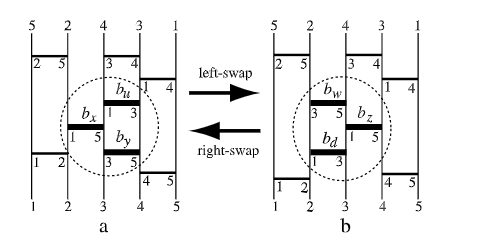
\includegraphics{LocalSwapOperation}
    }
    \caption{A local swap operation}
    \label{Fig:LocalSwap}
\end{figure}

In \emph{Optimal Reconfiguration of Optimal Ladder Lotteries}~\cite{A2}, written by Horiyama, Wasa and Yamanaka,
the authors provide a polynomial solution to the 
Minimal Reconfiguration Problem which asks, given 
two ladders, $L_{i}$ and  $L_{m}$, what is the minimal number of 
swap operations to perform that will transition from $L_{i}$ to $L_{m}$? A \emph{reverse triple} 
is a relation between three bars, $x,y,z$ in two arbitrary ladders, $L_{i}, L_{m}$, such that if $x,y,x$
are right swapped in $L_{i}$, then they are left swapped in $L_{m}$ or if they are 
left swapped in $L_{i}$ then they are right swapped in $L_{m}$. 
Let an \emph{improving triple} be defined as  
performing a right/left swapping three bars, $x,y,z$, in $L_{i}$ such that the 
result of the swap removes a reverse triple between
ladders $L_{i}$ and $L_{m}$. The improving triple is a symmetric 
relation, therefore performing a right/left swapping of the $x,y,z$ in $L_{m}$ also results in the 
removal of a reverse triple between $L_{i}$ and $L_{m}$.\par
The \emph{minimal length reconfiguration sequence} is the minimal number of 
improving triples required to transition from $L_{i}$ to $L_{m}$ or 
$L_{m}$ to $L_{i}$. Transitioning from $L_{i}$ to $L_{m}$ with the minimal length reconfiguration sequence 
is achieved by applying an improving triple to each of the reverse triples between 
$L_{i}$ and $L_{m}$. That is to say, the length of the reconfiguration sequence 
is equal to the number of improving triples required to remove all reverse triples between $L_{i}$ and  $L_{m}$.\par
The second contribution of this paper is that it provides a closed form formula for the 
upper bound for the minimal length reconfiguration sequence for any permutation 
of size $n$. That is to say, given some arbitrary $\pi$ of order $n$, what is the maximum 
number of swaps required for the minimal length reconfiguration sequence between any two ladders in $OptL\{\pi\}$?
The authors prove that there are two unique ladders in $OptL\{(n, n-1, \dots, 1)\}$ that 
have the upper bound for the minimal length reconfiguration sequence. These ladders are the root ladder and \emph{final ladder} 
which is defined as the unique ladder in $OptL\{\pi\}$ such that $\forall z < y < x: (y,z) \text{ is above } (x,z) \in l$. 
The length of the reconfiguration sequence 
between the root ladder and final ladder in $OptL\{(n, n-1, \dots, 1)\}$ is $n{n-1~\choose 2}$. 
\par

%%input review of fourth paper.

\subsection{Efficient Enumeration of all Ladder Lotteries with K Bars}

In this paper, the authors apply the same algorithm used in Efficient Enumeration of Optimal Ladder-Lotteries 
and its Application for generating all ladder lotteries with k bars \cite{A4}. The number of elements 
in The inversion set of $\pi$ also known as $Inv\{\pi\}$ provides the lower bound for $K$ 
and the upper bound is positive infinity. Therefore $K=[|Inv\{\pi\}| \dots N]$ \cite{A4}.\par\par 
\subsection{Coding Latter Lotteries}
\subsubsection{Overview}
In this paper, the authors provide three methods to encode ladder-lotteries as 
binary strings. Coding discrete objects as binary strings is an appealing theme because 
it allows for compact represntation of them for a computer \cite{A5}.
\subsubsection{Route Based Encoding}
The first method is termed \emph{route based encoding method} in 
which each route of an element in the permutation has a binary encoding. Let $L$
be a ladder-lottery for some arbitrary permutation $\pi$ of order $N$. The route 
of element $p_{i}$ is encoded by keeping in mind $p_{i}$ crosses bars in its route 
going left zero or more times and crosses bars in its route going right zero or 
more times \cite{A5}. The maximum number of bars $p_{i}$ can have is $N-1$, therefore the 
upper bound for the number of left/right crossings for $p_{i}$ is $N-1$ \cite{A5}. 
Let a left crossing be denoted with a $'0'$ and let a right crossing be denoted 
with a $'1'$. Let $C_{p_{i}}$ be the route encoding for the $i^{th}$ element 
in $\pi$. To construct $C_{p_{i}}$,  append $0$ and $1$ to each other representing 
the left and right crossings of $p_{i}$ from the top left 
to bottom right of the ladder \cite{A5}. If the number of crossings for $p_{i}$ 
is less than $n-1$, append $0s$ to the encoding of the route of $p_{i}$ until
the encoding is of length $N-1$ \cite{A5}. Let $LC_{L}$ be the route encoding for 
some arbitrary ladder in $OptL\{\pi\}$. $LC_{L}$ is $C_{p_{1}}, C_{p_{2}, \dots C_{p_{N}}}$.
For an example of the route encoding for the root ladder of $(3,2,5,4,1)$ refer to 
Fig.\ref{fig:route-encoding}. In \ref{fig:route-encoding}you will see that $C_{p_{1}}$ is 11\underline{00}. Underlined 
$0s$ are the $0s$ added to ensure the length of $C_{p_{1}}$ is $N-1$.
Since the length of $C_{pi}$ is $N-1$ and the number of elements in $\pi$ is $N$
then the length of $LC_{L}=N(N-1)$. Hence the number of bits needed for $LC_{L}$ 
belongs to $\mathcal{O}(N^{2})$.\par 
\begin{figure}[!htp]
    \begin{center}
        \begin{tikzpicture}
    
            %%draw the lines
            \draw(0, 0) to (0, 4);
                \node at(0, 4.3){3};
                \node at(0, -0.3){1};
            \draw(2, 0) to (2, 4);
                \node at (2, 4.3){2};
                \node at(2, -0.3){2};
            \draw(4, 0) to (4, 4);
                \node at (4, 4.3){5};
                \node at (4, -0.3){3};
            \draw(6, 0) to (6, 4);
                \node at (6, 4.3){4};
                \node at (6, -0.3){4};
            \draw(8, 0) to (8, 4);
                \node at (8, 4.3){1};
                \node at (8, -0.3){5};
    
            %%Draw the bars
            \draw(0, 2) to (2, 2);
            \draw(2, 1.5) to (4,1.5);
            \draw(0, 1) to (2, 1);

            \draw(4, 3) to (6, 3);
            \draw(6, 2.5) to (8, 2.5);
            \draw(4, 2) to (6, 2);
        \end{tikzpicture}
    \end{center}
   
 \caption{The route encoding for the following ladder lottery is 11\underline{00}01\underline{00}11\underline{00}01\underline{00}0000}
 \label{fig:route-encoding}

\end{figure}

\subsubsection{Line Based Encoding}
The second method is termed \emph{line based encoding} which focuses 
on encoding the lines of the ladder-lottery. Each line is represented 
as a sequence of endpoints of bars. Let $L$ be an optimal ladder-lottery 
with $N$ lines and $B$ bars, then for some arbitrary line, $i$, there 
are zero or more right/left endpoints of bars that 
come into contact with $i$ \cite{A5}. Let $LC_{i}$ denote the line based encoding for line $i$.
Let $1$ denote a left end point that 
comes into contact with line $i$ and let $0$ denote a right 
end point that comes into contact with line $i$. Finally, append a $0$
to line $i$ to denote the end of the line. Then line $i$ can be 
encoded, from top to bottom, as a sequence of $1s$ and $0s$ that 
terminates in a $0$.  Given the ladder in Fig. \ref{fig:line-encoding}, 
$LC_{3}$ is $001\underline{0}$. The \underline{0} denotes 
the end of the line. Let $LC_{L}$ be the line encoding for 
some arbitrary ladder, then $LC_{L}=LC_{1}, LC_{2}, \dots LC_{N}$.
Let $L_{(4,2,3,1)}$ refer to the ladder in Fig. \ref{fig:line-encoding}, then 
$LC_{L_{(4,2,3,1)}}=11\underline{0}010\underline{0}110\underline{0}010\underline{0}0\underline{0}$\par 
In order to reconstruct $L$ from its $LC_{L}$, or in other words decode
$LC_{L}$ it is important to recognize that the first line only has left endpoints attached to it
\cite{A5}. Since left end points are encoded as a $1$ then it is guarenteed that the first $0$ 
represents the end of line $1$. Secondly, the last/$Nth$ line 
has only right end points attached to it.  Therefore $LC_{N}$ will only have $0s$. Therefore, $LC_{N}$
does not require a terminating $0$. Thirdly, for any 
line $i+1$, if line $i+1$ has a $0$ then there must be a corresponding $1$
in line $i$. That is to say, if the right end point of a bar is on line 
$i+1$ then that same bar must have a left endpoint on line $i$. To decode 
$LC_{L}$ start by decoding line $1$. The line will contain $0$ or more 
left end points. To decode $LC_{i+1}$ where $i+1>1$, go to 
$LC_{i}$ and match each $1$ in $LC_{i}$ with a $0$ in $LC_{i+1}$. 
Let $k=$ the number of $1s$ in $LC_{i}$. Let $j=$ the number 
of $0s$ in $LC_{i+1}$ then $k=j-1$; due to the last $0$ in $LC_{i+1}$ denoting 
the end of line $i+1$.  Intuitively, this means match every left end point 
of a bar in line $i$ with a right end point in line $i+1$. The last $0$
represents the end of line $i+1$. For an example of a full decoding of $LC_{L_{(4,2,3,1)}}$
please refer to Fig. \ref{fig:line-encoding}.\pagebreak
\begin{figure}[!htp]
    \begin{center}
        \begin{tikzpicture}
            \draw(0, 0) to (0, 4);
            \node at (0, 4.3){4};
            \node at (0, -0.3){1};
        \draw(2, 0) to (2, 4);
            \node at (2, 4.3){2};
            \node at (2, -0.3){2};
        \draw(4, 0) to (4, 4);
            \node at (4, 4.3){3};
            \node at (4, -0.3){3};
        \draw(6, 0) to (6, 4);
            \node at (6, 4.3){1};
            \node at (6, -0.3){4};

        %%bars 
        \draw(0, 3) to (0.7, 3);
            \node at (0.35, 3.3){1};
        \draw (1.3, 3) to (2, 3);
            \node at (1.65, 3.3){0};

        \draw(2, 2.5) to (2.7, 2.5);
            \node at (2.35, 2.8){1};
        \draw(3.3, 2.5) to (4, 2.5);
            \node at (3.65, 2.8){0};

        \draw(4, 2) to (4.7, 2);
            \node at (4.35, 2.3){1};
        \draw(5.3, 2) to (6, 2);
            \node at (5.65, 2.3){0};

      

        \draw(2, 1) to (2.7, 1);
            \node at (2.35, 1.3){1};
        \draw(3.3, 1) to (4, 1);
            \node at (3.65, 1.3){0};

        \draw(0, 0.5) to (0.7, 0.5);
            \node at (0.35, 0.8){1};
        \draw(1.3, 0.5) to (2, 0.5);
            \node at (1.65, 0.8){0};

        \end{tikzpicture}
      

    \end{center}
    \caption{$LC_{L(4,2,3,1)}=LC_{1}=11\underline{0},LC_{2}=0110\underline{0},LC_{3}=010\underline{0},LC_{4}=0$}
    \label{fig:line-encoding}
\end{figure}

Since each bar is encoded as two bits, and there are $N-1$ bits as terminating bits; 
one for each line in $L$, then the number of bits required is $N + 2B -1$, where $N$
is the number of lines and $B$ is the number of bars. Encoding and decoding can be 
done in $\mathcal{O}(n+b)$ time.\cite{A5} Clearly the line-based encoding 
trumps the route-based encoding in both time and space complexity.

\subsubsection{Improved Line-Based Encoding}
Although the line-based encoding is better than the route based 
encoding, it can still be further optimized. The authors provide 
three improvements to the line-based encoding. These three improvements
can be combined to really help imrpove the line based encoding's 
space efficiency \cite{A5}. 
\paragraph{Imrpovement 1}
Since the $Nth$ line has only right endpoints attached to it, 
then it actually does not need to be encoded. Right endpoints 
are denoted as $0$ and left endpoints are encoded as $1$, therefore the number of right endpoints 
for line $N$ is equal to the number of $1s$ in $LC_{N-1}$.
Thus, there is no need for $LC_{N}$ \cite{A5}. The encoding with improvment 
one for the ladder in Fig. \ref{fig:line-encoding} is $11\underline{0}0110\underline{0}010$.
\paragraph{Improvement 2}
Improvement two is based off of the fact that for any two bars,
$x,y$, let $l_{x}$ denote the left endpoint of bar $x$, let 
$l_{y}$ denote the left endoint of bar $y$, let $r_{x}$ denote 
the right end point of bar $x$ and let $r_{y}$ denote the right 
end point of bar $y$. Let line $i$ be the line of $l_{x}$ and $l_{y}$
and let line $i+1$ be the line of $r_{x}$ and $r_{y}$.
\begin{lemma}
There are three possible cases for the 
placement of $x$ and $y$ in some 
arbitrary ladder from $OptL\{\pi\}$. The first case is that there 
is at least one other bar, $z$, with a right end point, $r_{z}$ between $l_{x}$
and $l_{y}$ on line $i$. The second case is that there is at least one other bar 
$z$, with a left end point, $l_{z}$, between $r_{x}$ and $r_{y}$ on line $i+1$. 
The third case is that there is at least one bar, $z$, with a right end point, 
$r_{z}$, betwen $l_{x}$ and $l_{y}$ on line $i$ and there is at least one other bar, 
$z\prime$ with a left end point, $l_{z\prime}$, between $r_{x}$ and $r_{y}$ on line $i+1$ \cite{A5}. 
For an example of all three cases refer to Fig. \ref{fig:three-cases}\par
\end{lemma}

%%figure demonstrating the three cases for bar positions
\begin{figure}[!htp]
       
            %%first case
            \begin{minipage}{.3\textwidth}
                \begin{tikzpicture}
                    \draw(0, 0) to (0, 4);
                        \node at (2, 4.3){\small{$i+1$}};
                    \draw(1, 0) to (1, 4);
                        \node at (1, 4.3){\small{$i$}};
                    \draw(2, 0) to (2, 4);
                        \node at (0, 4.3){\small{$i-1$}};
                    \draw(0, 2) to (1, 2);
                        \node at (.5, 2.3){\small{$r_{z}$}};
                    \draw(1, 3) to (2, 3);
                        \node at (1.5, 3.3){\small{$l_{x}$}};
                    \draw(1, 1) to (2, 1);
                        \node at (1.5, 1.3){\small{$l_{y}$}};
                \end{tikzpicture}
            \end{minipage}
              \begin{minipage}{.3\textwidth}

                 \begin{tikzpicture}
                
                  \draw(0, 0) to (0, 4);
                     \node at (0, 4.3){\small{$i-1$}};
                  \draw(1, 0) to (1, 4);
                    \node at (1, 4.3){\small{$i$}};
                  \draw(2, 0) to (2, 4);
                     \node at (2, 4.3){\small{$i+1$}};
                   \draw(0, 3) to (1, 3);
                         \node at (.5, 3.3){\small{$r_{x}$}};
                    \draw(1, 2) to (2, 2);
                         \node at (1.5, 2.3){\small{$l_{z}$}};
                     \draw(0, 1) to (1, 1);
                         \node at (0.5, 1.3){\small{$r_{y}$}};
                
                   
                
                \end{tikzpicture}
             \end{minipage}
             \begin{minipage}{.3\textwidth}

                \begin{tikzpicture}
                
                 \draw(0, 0) to (0, 4);
                    \node at (1, 4.3){\small{$i$}};
                 \draw(1, 0) to (1, 4);
                    \node at (2, 4.3){\small{$i+1$}};
                 \draw(2, 0) to (2, 4);
                    \node at (0, 4.3){\small{$i-1$}};
                 \draw(3, 0) to (3, 4);
                    \node at (3, 4.3){\small{$i+2$}};
                    \draw(1, 3) to (2, 3);
                        \node at (1.3, 3.3){\small{$l_{x}$}};
                        \node at (1.7, 3.3){\small{$r_{x}$}};
                     \draw(0, 2) to (1, 2);
                        \node at (0.7, 2.3){\small{$r_{z}$}};
                    \draw(1, 1) to (2, 1);
                        \node at (1.3, 1.3){\small{$l_{y}$}};
                         \node at (1.7, 1.3){\small{$r_{y}$}};
                     \draw(2, 2) to (3, 2);
                        \node at (2.3, 2.3){\small{$l_{z\prime}$}};
                
                   
                
                \end{tikzpicture}
            \end{minipage}
        

    \caption{Three examples of the three cases for the placement 
    of bars $x$ and $y$ in a ladder-lottery}
    \label{fig:three-cases}
\end{figure}
\begin{proof}
    Suppose that none of the above cases hold. Let $L_{\pi}$ be an 
    optimal ladder-lottery with bars $x$ and 
    bar $y$. If none of the cases hold then $x$ and $y$ are directly above/below each other without 
    the enpoint of some third bar $z$ between $l_{x}$ and $l_{y}$ or between $r_{x}$ and $r_{y}$.
    Let $x$ be the bar for the inversion of two elements $p$ and $q$ in $\pi$. 
    As $p$ and $q$ travel through the ladder they will cross each other at bar $x$; 
    thus uninverting them. Since bar $y$ is directly below bar $x$, then $p$ and $q$ will cross 
    bar $y$ thus re-inverting them. Therefore, there will need to be a third 
    bar that uninverts $p$ and $q$ a second time. Since this third bar is 
    redundant, $L_{\pi}$ is non-optimal which is a contradiction. Let $x$ be a bar for two 
    elements in $\pi$, $p$ and $q$ such that $p$ and $q$ do not form an inversion. Then $x$ 
    will invert $p$ and $q$ and $y$ will uninvert them. Thus making both $x$ and $y$ redundant
    bars which is also a contradiction. Therefore one of the above cases must hold.
\end{proof}
Knowing that one of the three above cases must hold is beneficial for improving the 
line-based encoding. If $l_{x}$ and $l_{y}$ on line $i$ have no $r_{z}$ between them, 
then there must be at least one $l_{z\prime}$ between $r_{x}$ and $r_{y}$ on line $i+1$.
Since a left endpoint is encoded as a $1$ and a right endpoint is encoded as a $0$, 
a $1$ can be omitted for the encoding of line $i+1$ if $l_{x}$ and $l_{y}$ have no $r_{z}$
between them on line $i$ \cite{A5}. That is to say, if there is not a $0$ between 
the two  $1s$ for $l_{x}$, $l_{y}$ in $LC_{i}$, it is implied that there is at least one $1$ between 
the two $0s$ for $r_{x}$, $r_{y}$ on $LC_{i+1}$. Hence, one of the $1s$ in $LC_{i+1}$ can be omitted. 
The line encoding with improvement two for the ladder in Fig. \ref{fig:line-encoding} is $11\underline{0}010\underline{0}00\underline{0}0$.
\paragraph{Imrpovement 3}
Improvement three is based off of saving some bits for right 
end points/$0s$ in $LC_{N-1}$. Since line $N$ has no left end points,
then then there must be some right endpoints between any two 
consecutive bars connecting lines $N-1$ and line $N$. If you 
refer to Fig. \ref{fig:improvement3}, then the only configuration for lines $N-2, N-1, N$
is the middle configuration \cite{A5}. Knowing this, then 
given two bars, $x$ and $y$ with $l_{x}$/$l_{y}$ on line 
$n-1$ and $r_{x}$/$r_{y}$ on line $n$, there must be at least 
one bar, $z$, with its $r_{z}$ between $l_{x}$ and $l_{y}$
on line $N-1$. Thus, for every $1$ in $LC_{N-1}$ except the 
last $1$ in $LC_{N-1}$, a $0$ must immidediately proceed any $1$
in $LC_{N-1}$. Since this $0$ is implied, it can be removed from $LC_{N-1}$ \cite{A5}. 
For an example of improvement three with its line encoding for $LC_{N-1}$ please refer to Fig.\ref{fig:improvement3}\pagebreak
\begin{figure}[!htp]
    \centering
    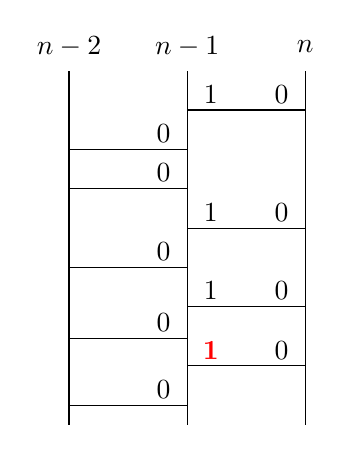
\begin{tikzpicture}
        \draw(0, -0.5) to (0, 4);
            \node at (0, 4.3){$n-2$};
            \draw(0, 3) to (1.5, 3);
                \node at (1.2, 3.2){$0$};
            \draw(0, 2.5) to (1.5, 2.5);
                \node at (1.2, 2.7){$0$};
            \draw(0, 1.5) to (1.5, 1.5);
                \node at (1.2, 1.7){$0$};
            \draw(0, 0.6) to (1.5, 0.6);
                 \node at (1.2, 0.8){$0$};
            \draw(0, -0.25) to (1.5, -0.25);
                \node at (1.2, -0.05){$0$};
        \draw(1.5, -0.5) to (1.5, 4);
            \node at (1.5, 4.3){$n-1$};
            \draw(1.5, 3.5) to (3, 3.5);
                \node at (1.8, 3.7){$1$};
                \node at (2.7, 3.7){$0$};
            \draw(1.5, 2) to (3, 2);
                \node at (1.8, 2.2){$1$};
                \node at (2.7, 2.2){$0$};
            \draw(1.5, 1) to (3, 1);
                \node at (1.8, 1.2){$1$};
                \node at (2.7, 1.2){$0$};
            \draw(1.5, 0.25) to (3, 0.25);
                \node at (1.8, 0.45){$\textcolor{red}{\textbf{1}}$};
                \node at (2.7, 0.45){$0$};

        \draw(3, -0.5) to (3, 4);
            \node at (3, 4.3){$n$};
    \end{tikzpicture}
    \caption{The line coding for $LC_{N-1}$ with imrpovement three is $101110$\underline{$0$}. The red, bold $1$ represents 
    the last left end point in $LC_{N-1}$, therefore the proceeding $0$ must be 
    included in $LC_{N-1}$. For every other $1$ in $LC_{N-1}$, a $0$ is omitted following 
    said $1$.}
    \label{fig:improvement3}
\end{figure}
\paragraph{Combining All Three}
The combination of all three improvements can be done independently. 
Let $IC_{L_{(4,2,3,1)}}$ be the \emph{improved line-based encoding} for $L_{(4,2,3,1)}$ 
by applying improvements 1-3 to $LC_{L_{(4,2,3,1)}}$. Recall that $LC_{L}$ denotes the line-based encoding for some ladder $L$.
$LC_{L_{(4,2,3,1)}}$ for the ladder in Fig. \ref{fig:line-encoding} is $11\underline{0}10101\underline{0}0010101\underline{0}000$.
By applying imrpovement one, we get $11\underline{0}101011\underline{0}0010101\underline{0}$. 
Notice how the last three $0s$ from $LC_{L}$ were removed because they represented $LC_{N}$.
By applying imrpovement two to improvememt one we get $11\underline{0}10011\underline{0}001001\underline{0}$.
Notice how the second, and eigth $1$ were removed because they are implied by 
the successive $0s$. By applying improvement three to the result of improvement 
two we get $11\underline{0}10011\underline{0}00101\underline{0}$. Notice how the last $0$ 
was removed from improvement two. This is because the $0$ is implied in $LC_{N-1}$
due to the configuration between of bars connecting lines $N-1$ and line $N$. The $IC_{L_{(4,2,3,1)}}$ for the ladder in fig. \ref{Fig:allthree} 
is $IC_{L_{(4,2,3,1)}}=11\underline{0}10011\underline{0}00101\underline{0}$.\pagebreak

\begin{figure}[!htp]
     \centering
    \begin{tikzpicture}
         \draw(0, 0) to (0, 4);
             \node at (0, 4.3){$n-3$};
             \draw(0, 3.5) to (1.5, 3.5);
             \draw(0, 2.5) to (1.5, 2.5);
         \draw(1.5, 0) to (1.5, 4);
             \node at (1.5, 4.3){$n-2$};
             \draw(1.5, 3) to (3, 3);
             \draw(1.5, 3.8) to (3, 3.8);
             \draw(1.5, 2) to (3, 2);
             \draw(1.5, 1) to (3, 1);
         \draw(3, 0) to (3, 4);
             \node at(3, 4.3){$n-1$};
             \draw(3, 2.5) to (4.5, 2.5);
             \draw(3, 1.5) to (4.5, 1.5);
             \draw(3, 0.5) to (4.5, 0.5);
         \draw(4.5, 0) to (4.5, 4);
             \node at(4.5, 4.3){$n$};
     \end{tikzpicture}
     \caption{A ladder used to illustrate all three improvements $IC_{L}$. $IC_{L}=11\underline{0}10011\underline{0}00101\underline{0}$}
     \label{Fig:allthree}
\end{figure}
\section{Enumeration, Counting, and Random Generation of \newline Ladder Lotteries}

In the paper, Enumeration, Counting, and Random Generation of Ladder Lotteries~\cite{A6}, written by Nakano and Yamanaka 
the authors consider the problem of enumeration, counting and 
random generation of ladder lotteries with $n$ lines and $b$ bars. 
It is important to note that the authors considered both optimal and 
non-optimal ladders for this paper. Nonetheless, the paper is still fruitful 
for its modelling of the problems and insights into ladder lotteries.
The authors use  the line-based encoding, $LC(l)$ for the representation of ladders 
that was discussed in the review of Coding Ladder Lotteries~\cite{A5}.

%%Section for enumeration
\subsection{Enumeration}
The authors denote a set of ladder lotteries with $n$ lines and 
$b$ bars as $S_{n,b}$. The problem is how to enumerate all the 
ladders in $S_{n,b}$. The authors use a \emph{forest structure}
to model the problem. A \emph{forest structure} is a set of trees 
such that each tree in the forest is disjoint union with every other 
tree in the forest. Consider $S_{n,b}$ to be a tree in a forest.
That is to say, a union disjoint subset of all ladders with $n$
lines and $b$ bars. Then $F_{n,b}$, or the forest of all $S_{n,b}$,
is the union of all disjoint trees of ladders with $n$ lines and $b$ bars. 
%For an example 
% of a forest for $F_{3,2}$ refer to Figure~\ref{fig:forest3,2}.\pagebreak %figure number.
% \begin{figure}[t]
%     \begin{center}
%     \begin{minipage}{.8\textwidth}
%         \begin{tikzpicture}
%             \draw(0, 0) to (0, 2);
%             \draw(0.5, 0) to (0.5, 2);
%                 \node at(0.25, -0.5){00};

%             %%branch
%             \draw[line width=0.5mm] (0.8, 1) to (1.3, 1);

%             \draw(1.5, 0) to (1.5, 2);
%                 \draw(2, 1.5) to (2.25, 1.5);
%             \draw(2, 0) to (2, 2);
%                 \node at (1.75, -0.5){0\underline{1}0};
    
%             %%branch
%             \draw[line width=0.5mm] (2.3, 1) to (2.8, 1);
            
%             \draw(3, 0) to (3, 2);
%             \draw(3.5, 0) to (3.5, 2);
%                  \draw(3.5, 1.5) to (3.75, 1.5);
%                  \draw(3.5, 1) to (3.75, 1);
%                 \node at (3.25, -0.5){01\underline{1}0};
            
%             \draw[line width=0.5mm] (4, 1) to (4.5, 1);

%             \draw(4.6, 0) to (4.6, 2);
%             \draw(5.1, 0) to (5.1, 2);
%             \draw(5.6, 0) to (5.6, 2);
%                  \draw(5.1, 1.5) to (5.35, 1.5);
%                  \draw(5.1, 1) to (5.35, 1);
%                 \node at (5.1, -0.5){011\underline{0}0};


%             \draw[line width=0.5mm](5.8, 1) to (6.3, 1);
%             \draw(6.5, 0) to (6.5, 2);
%             \draw(7, 0) to (7, 2);
%             \draw(7.5, 0) to (7.5, 2);
%                 \draw(7, 1.5) to (7.5, 1.5);
%                 \draw(7, 1) to (7.25, 1);
%                 \node at (7, -0.5){0110\underline{0}0};

%             \draw[line width=0.5mm](7.8, 1) to (8.3, 1);
%             \draw(8.6, 0) to (8.6, 2);
%             \draw(9.1, 0) to (9.1, 2);
%             \draw(9.6, 0) to (9.6, 2);
%                 \draw(9.1, 1.5) to (9.6, 1.5);
%                 \draw(9.1, 1) to (9.6, 1);
%                 \node at (9.1, -0.5){01100\underline{0}0};

%         \end{tikzpicture}
        
%     \end{minipage}
%     \end{center}
    
    
  

%     %%second tree
%     \begin{center}
%           \begin{minipage}{0.8\textwidth}
%             \begin{tikzpicture}
%                 \draw(0, 0) to (0, 2);
%                 \draw(0.5, 0) to (0.5, 2);
%                     \draw(0, 1) to (0.25, 1);
%                     \node at (0.25, -0.5){$100$};
                
%                 %%upper subtree
%                 \draw[line width=0.5mm](0.8, 1.5) to (1.3, 2);
%                     \draw(1.5, 1.5) to (1.5, 3.5);
%                     \draw(2, 1.5) to (2, 3.5);
%                         \draw(1.5, 3) to (2, 3);
%                         \node at (1.75, 1){$10\underline{0}0$};

%                     \draw[line width=0.5mm](2.3, 2.5) to (2.8, 2.5);
%                         \draw(3, 1.5) to (3, 3.5);
%                             \draw(3, 3) to (3.5,3);
%                             \draw(3.5, 2.5) to (3.75, 2.5);
%                         \draw(3.5, 1.5) to (3.5, 3.5);
%                         \node at (3.5, 1){$100\underline{1}0$};

%                     \draw[line width=0.5mm](4, 2.5) to (4.5, 2.5);
%                         \draw(4.7,  1.5) to (4.7, 3.5);
%                             \draw(4.7, 3) to (5.2, 3);
%                             \draw(5.2, 2.5) to (5.45, 2.5);
%                         \draw(5.2, 1.5) to (5.2, 3.5);
%                         \draw(5.7, 1.5) to (5.7, 3.5);
%                         \node at (5.2, 1){$1001\underline{0}0$};

%                     \draw[line width=0.5mm](6, 2.5) to (6.5, 2.5);
%                         \draw(6.8,  1.5) to (6.8, 3.5);
%                             \draw(6.8, 3) to (7.3, 3);
%                             \draw(7.3, 2.5) to (7.8, 2.5);
%                         \draw(7.3, 1.5) to (7.3, 3.5);
%                         \draw(7.8, 1.5) to (7.8, 3.5);
%                         \node at (7.3, 1){$10010\underline{0}0$};



%                 %%lower subtree
%                 \draw[line width = 0.5mm](0.8, 0.5) to (1.3, 0);
%                     \draw (1.5, -0.5) to (1.5, -2.5);
%                         \draw(1.5, -1.5) to (1.75, -1.5);
%                         \draw(2, -1) to (2.25, -1);
%                     \draw(2, -0.5) to (2, -2.5);
%                         \node at (1.5, -2.8){$10\underline{1}0$};
                    
%                     \draw[line width = 0.5mm](2.55, -1.5) to (3.05, -1.5);

%                      \draw (3.3, -0.5) to (3.3, -2.5);
%                         \draw(3.3, -1.5) to (3.8, -1.5);
%                         \draw(3.8, -1) to (4.05, -1);
%                     \draw(3.8, -0.5) to (3.8, -2.5);
%                         \node at (3.6, -2.8){$101\underline{0}0$};

%                      \draw[line width = 0.5mm](4.25, -1.5) to (4.75, -1.5);

%                      \draw (5, -0.5) to (5, -2.5);
%                         \draw(5.5, -1) to (5.75, -1);
%                         \draw(5, -1.5) to (5.5, -1.5);
%                     \draw(5.5, -0.5) to (5.5, -2.5);
%                     \draw(6, -0.5) to (6, -2.5);
%                         \node at (5.5, -2.8){$1010\underline{0}0$};
                    

%                     \draw[line width = 0.5mm](6.3, -1.5) to (6.8, -1.5);
%                     \draw (7.1, -0.5) to (7.1, -2.5);
%                         \draw(7.1, -1.5) to (7.6, -1.5);
%                         \draw(7.6, -1) to (8.1, -1);
%                     \draw(7.6, -0.5) to (7.6, -2.5);
%                     \draw(8.1, -0.5) to (8.1, -2.5);
%                         \node at (7.6, -2.8){$10100\underline{0}0$};
                    

                    
%             \end{tikzpicture}
            
%         \end{minipage}
%     \end{center}


%     \begin{center}
%         \begin{minipage}{0.8\textwidth}
%             \begin{tikzpicture}%% start pocture
            
            
%                 \draw(0, 0) to (0, 2);
%                     \draw(0, 1.5) to (0.25, 1.5);
%                     \draw(0, 1) to (0.25, 1);
%                 \draw(0.5, 0) to (0.5, 2);
%                 \node at (0.25, -0.5){$1100$};
            
            
%                 \draw[line width=0.5mm] (0.8, 1) to (1.3, 1);
%                     \draw(1.5, 0) to (1.5, 2);
%                         \draw(1.5, 1.5) to (2, 1.5);
%                         \draw(1.5, 1) to (1.75, 1);
%                     \draw(2, 0) to (2, 2);
%                     \node at (1.75, -0.5){$110\underline{0}0$};
            
        
%                 \draw[line width=0.5mm] (2.3, 1) to (2.8, 1);
%                     \draw(3, 0) to (3, 2);
%                        \draw(3, 1.5) to (3.5, 1.5);
%                        \draw(3, 1) to (3.5, 1);
%                    \draw(3.5, 0) to (3.5, 2);
%                     \node at (3.25, -0.5){$1100\underline{0}0$};
            
            
%                 \draw[line width=0.5mm] (3.8, 1) to (4.3, 1);
%                     \draw(4.5, 0) to (4.5, 2);
%                           \draw(4.5, 1.5) to (5, 1.5);
%                           \draw(4.5, 1) to (5, 1);
%                       \draw(5, 0) to (5, 2);
%                       \draw(5.5, 0) to (5.5, 2);
%                           \node at (5, -0.5){$11000\underline{0}0$};
               
%             \end{tikzpicture}%%end picture
%         \end{minipage}
%     \end{center}
%     \caption{The forest, $F_{3,2}$ where $3$ is the number of lines and $2$ is the number of bars. All ladders with $3$ lines and $2$ bars are leaf nodes of one of three trees $S_{3,2}$.
%     The underlined bits are the inserted second last bit from the parent's line-encoding resulting in the child's line encoding}
%     \label{fig:forest3,2}
% \end{figure}

%%end enumeratiom section

%%section for counting
\subsection{Counting}
The authors provide a method and algorithm to count all ladders 
with $n$ lines and $b$ bars. The counting algorithm 
works by dividing ladders into four types of sub-ladders.
For sub-ladder, $r$, its type is a tuple $t(n,h,p,q)$ where 
$n$ is the number of lines, $h$ is the number of half bars, 
$p$ is the number of unmatched end-points on line $n-1$ and 
$q$ is the number of unmatched end-points on line $n$. From this 
type, the authors are able to count all ladders with $n$ lines and $b$ bars. 
% \subsubsection{ $h < p+q$ or $n<2$}
% There are zero ladders because it is impossible for the 
% root sub-ladder to have less than two lines. It is also 
% impossible for the number of half bars, $h$, to 
% be less than the number of detached left end points 
% on line $n-1$ plus the number of detached end points on 
% line $n$.

% %%\subsubsubsection{Case 2: $n=2$ and $h=p$ and $q=0$}
% \subsubsection{$n=2$ and $h=p$ and $q=0$}
% There is only one ladder because the number of half bars 
% on the last line is 0 since $q=0$. Therefore all half bars are on the 
% $n-1th$ line of the sub-ladder. This is known because 
% $h=p$ which means the number of half bars is the same as 
% the number of unmatched bars on line $n-1$. Hence, the unmatched 
% half bars on the $n-1th$ line must be connected to the $n$ 
% line. Once these are all matched the ladder will be complete. 
% Thus, there is only one ladder for this case.

% %%\subsubsubsection{Case 3: $(n \geq 3$ or $h>p)$ and $q=0$}
% \subsubsection{$(n \geq 3$ or $h>p)$ and $q=0$}
% If this is the case, then there are no endpoints attached to 
% line $n$, but the number of half bars is greater than the 
% number of endpoints attached to line $n-1$, which means there is 
% some line(s) $n-t$, $t>2$ that have end points attached to them.
% Let $r$ be a sub-ladder of type $r=t(n,h,p,q)$
% with the the above values for $n,h,p,q$. In order to count the number of ladders of type 
% $t(n\geq3, h>p, q=0)$ the authors demonstrate an injection $|t(n\geq3, h>p, q=0)|=|t(n-1,h,0,p)| + |t(n,h-1,p+1,q)|$.\cite{A6}
% Let $P(r)$ be $r$ with the removal of $r's$ second last bit in $LC(r)$; i.e. the parent of 
% $r$.  The $LC(r)$ must have a $0$ for the second last bit. This $0$ designates either the 
% end of line $n-1$ or a right endpoint of a bar attached to line $n-1$. 
% If the second last bit in $LC(r)$ is the right end point of some 
% bar, then $P(r)=t(n,h-1,p+1,q)$. This is because the $n-1th$ bar 
% has a right end point that must be connected to some left  
% endpoint at line $n-2$. Since the removal sequence of the second 
% last bit ensures that there cannot be a right end-point detached 
% from a left end-point. Only left end-points can be detached 
% from right end-points~\cite{A6}. However, if the second last bit 
% of $LC(r)$ designates the end of line $n-1$, then $P(r)=t(n-1,h,0,p)$. 
% This is because the removal of the second last bit 
% is the removal of the end of line $n-1$ in $r$. Thus, 
% line $n$ must be empty in $r$ since the last bit in $LC(r)$
% designated the end of line $n$. Thus, if line $n$ is empty 
% and the end point of line $n-1$ has been removed from $LC(r)$, 
% resulting in $P(LC(r))$, the last bit in $P(LC(r))$ must be 
% the end of line $n-1$ in $r$ resulting in a pre-ladder with one 
% less line than $r$.\par  

% \subsubsection{ $h\geq p+q$ and $q>0$}
% %%\subsubsubsection{Case 4: $h\geq p+q$ and $q>0$}
% Let $r$ be a pre-ladder of type $t(n,h,p,q)$. The authors 
% demonstrate $|t(n,h\geq p+q,q>0)|=|t(n,h-1,p+1,q)|+|t(n,h-1,p,q-1)|$.\cite{A6} 
% The second last bit of $LC(r)$ is either a $0$ 
% or a $1$. If it is a $0$ then it represents a 
% right end point attached to line $n$. Thus, 
% removing it to get $P(LC(r))$ is in effect 
% detaching a right end point from some left end point 
% on line $n-1$. Therefore, the parent, $P(R)$ is 
% of type $t(n,h-1,p+1,q)$. Seeing as in the parent, 
% there is now a left end point detached from its right 
% end point in $r$. However, if the second last bit 
% of $LC(r)$ is a $1$, then this indicates the left 
% half of a bar on line $n$. But since there is no 
% bar $n+1$, this left end point must be detached. 
% Therefore, by removing this $1$ in $LC(r)$ results 
% in a parent with one less detached end point on line $n$.
% Thus $P(R)$ is of type $t(n,h-1,p,q-1)$.
% \subsection{Random Generation}
% The random generation of ladder lotteries with $n$ lines and
% $b$ bars is done by the recurrence relations in the counting 
% and enumerating sections. The goal is to produce 
% some $L$ of type $t(n,2b,0,0)$ where the number of half 
% bars equals the total $2(b)$ and there are no detached 
% end points on lines $n-1$ and $n$. This implies that there 
% are no detached endpoints on any line $n-t$ where $t\geq2$
% because the removal sequence from the $LC(pre-ladder)$
% ensures that any line before $n-1$ has no detached endpoints. Thus, 
% if $L$ is of type $t(n,2b,0,0)$ it is no longer a pre-ladder 
% but a complete ladder with $n$ lines and $b$ bars~\cite{A6}.\par 
% The authors use an algorithm to generate a random integer, $x$,
% in the range of $[1 \dots |t(n,h,p,q)|]$. where $t(n,h,p,q)$ corresponds to some 
% parent type of ladder. $t(n1,h1,p1,q1)$ corresponds to one 
% child type of $t(n,h,p,q)$ and $t(n2,h2,p2,q2)$ corresponds 
% to the other child type. If $x\leq|t(n1,h1,p1,q1)|$ then generate 
% a pre-ladder of type $t(n1,h1,p1,q1)$ else generate a pre-ladder 
% of type $t(n2,h2,p2,q2)$~\cite{A6}. Continue until there is type $t(n,2b,0,0)$
% which corresponds to a complete ladder lottery with $n$ lines and $b$ bars.

%%%section on how ladde lotteries relate to other mathematical objects
% Despite the fact that ladder lotteries have only been stuidied in and
% of themseleves for ten years, they are closely tied to other mathematical 
% phenomena that have been studied for much longer. These mathematical phenomena  
%  include \emph{Pseudo Lines} which are an arrangement of 
% curves on a plane such that given two curves, they only intersect 
% at most once and at each intersection, only two curves intersect.See figure --reference--
% for a wiring diagrams of the pseudo line arrangement for the 
% permutation, $(5,4,3,2,1)$. The other mathematical phenomena is \emph{adjacent transpositions}
% which is a swap of two adjacent elements in a permutation. 
%%\subsection{Ladders and Adjacent Transpositions}
A ladder lottery is a way of sorting a permutation, yet it can also be thought of as 
a decomposition of a permutation into \emph{adjacent transpositions}. \cite{A1} 
An \emph{adjacent transposition} is simply a swap of two adjacent elements in a 
permutation. For example, given the permutation (1, 3, 4, 2), an adjacent 
transposition could be done on the following pairs of elements: 
(1, 3), (3, 4) or (4, 2). Each would result in a unique permutation. 
Simply put, given any arbitrary starting permutation, $\pi$, keep swapping 
adjacent inversions until the identity permutation is reached.  An optimal 
ladder lottery from $\pi's$ optimal ladder set is a minimal sequence of 
adjacent transpositions such that $\pi$ is sorted into the identity permutation; 
each ladder in the set represents a sequence of adjacent transpositions for 
sorting $\pi$ into the identity permutation. For example, given the permutation 
(4, 3, 2, 1) there exists eight ladders in this permutation's optimal ladder set. 
Two of these ladders are found in \ref{fig:ac}:

\begin{figure}[!htp]
    \label{fig:ac}
	\begin{minipage}{0.4\textwidth}
		\centering
	
		\begin{tikzpicture}
			\draw(0, 0) to (0, 4) node[above]{4};
			\draw(2, 0) to (2, 4) node[above]{3};
			\draw(4, 0) to (4, 4) node[above]{2};
			\draw(6, 0) to (6, 4) node[above]{1};
			
			\draw(0, 3.7) to (2, 3.7);
				\draw node at (1, 3.9) {(4, 3)};
			\draw(2, 3.25) to (4, 3.25);
				\draw node at (3, 3.45){(4, 2)};
			\draw(4, 2.75) to (6, 2.75);
				\draw node at (5, 3.0){(4, 1)};
			
			\draw(0, 2.75) to (2, 2.75);
				\draw node at (1, 3.0){(3, 2)};
			\draw(2, 2.25) to (4, 2.25);
				\draw node at (3, 2.5){(3, 1)};
			
			
			\draw(0, 1.75) to (2, 1.75);
				\draw node at (1, 1.95){(2, 1)};
			
			\draw node at (0, -0.5){1};
			\draw node at (2, -0.5){2};
			\draw node at (4, -0.5){3};
			\draw node at (6, -0.5){4};
			
			%%second ladder%%
			\draw(9, 0) to (9, 4) node[above]{4};
			\draw(11, 0) to (11, 4)node[above]{3};
			\draw(13, 0) to (13, 4)node[above]{2};
			\draw(15, 0) to (15, 4)node[above]{1};
			
			\draw(9, 3.7) to (11, 3.7);
				\draw node at (10, 3.9) {(4, 3)};
			\draw(11, 3.25) to (13, 3.25);
				\draw node at (12, 3.45){(4, 2)};
			\draw(13, 2.75) to (15, 2.75);
				\draw node at (14, 3.0){(4, 1)};
			
			\draw(9, 1.25) to (11, 1.25);
				\draw node at (10, 1.5){(3, 1)};
			\draw(11, 2) to (13, 2);
				\draw node at (12, 2.25){(2, 1)};
			
			\draw(11, 0.65) to (13, 0.65);
				\draw node at (12, 0.85){(3, 2)};
			 
			
			\draw node at (9, -0.5){1};
			\draw node at (11, -0.5){2};
			\draw node at (13, -0.5){3};
			\draw node at (15, -0.5){4};	
		\end{tikzpicture}
	
	\end{minipage}
	

	
		
	\caption{The left ladder is one of eight unique ladders from (4,3,2,1)'s optimal ladder set. The right ladder is another one of eight unique ladders form (4,3,2,1)'s optimal ladder set}
		
\end{figure}

From looking at the above ladders, going from top left to bottom right, the left ladder represents the sequence of adjacent transpositions (4,3), (4,2), (4,1),(3,2),(3,1),(2,1) 
whereas the right ladder represent the sequence of adjacent transpositions 
(4, 3),(4, 2),(4, 1),(2, 1),(3, 1),(3, 2). 
Notice how the length of the sequences are the same,because both lengths are equal 
to the minimal number of swaps to sort (4, 3, 2, 1) 
it is simply the order in which the adjacent transpositions occur in the sequence 
that makes the sequences different from each other. 